\chapter{直线形}

在第一章里,我们从日常生活所熟悉的位置、通路、方
向、叠合出发,讨论了空间的几个重要的基本概念:点、直
线、平行、全等、相似,并通过观察、实验,分析归纳出了
空间的一些性质。在第二章中,我们把其中的某些性质作为
基本性质和定理。在本章中,我们将以这些基本性质和定理
为基础,运用第二章所介绍的演绎法去推演空间的其它性
质。演绎法不但是研究几何学的基本有效方法,在其它任何
科学的研究中也都是十分重要的方法。概括地说,对于科学
研究,实验归纳和论证推演是互相配合使用的两种基本科学
方法,它们是探索科学规律的两条腿。从这一章起,我们对
空间性质的探讨,主要用演绎法来进行。
\section{三角形}

\subsection{全等三角形}

\begin{blk}{定义}
    平面上顺次首尾端点相接且不在同一条直线上的
线段组成的封闭图形叫做\textbf{多边形}。这些线段叫做\textbf{多边形的边},
它们的端点叫做\textbf{多边形的顶点},每相邻两边的夹角叫做多边
形的\textbf{内角}。
\end{blk}


三角形是多边形中最简单的图形。有四条边的多边形叫
做四边形,有五条边的多边形叫五边形……等等。表示一个
多边形可用顶点的名称,沿周界顺次列出,如图3.1中的
$\triangle ABC$,四边形$ABCD$……等等。

如果多边形都在每边所在直线的同旁,我们称这种多边
形为\textbf{凸多边形}(图3.1中的三个图形都是凸多边形,图3.2
中的图形则不是)。以后我们说多边形时,都指的是凸多边
形。
\begin{figure}[htp]
    \centering
    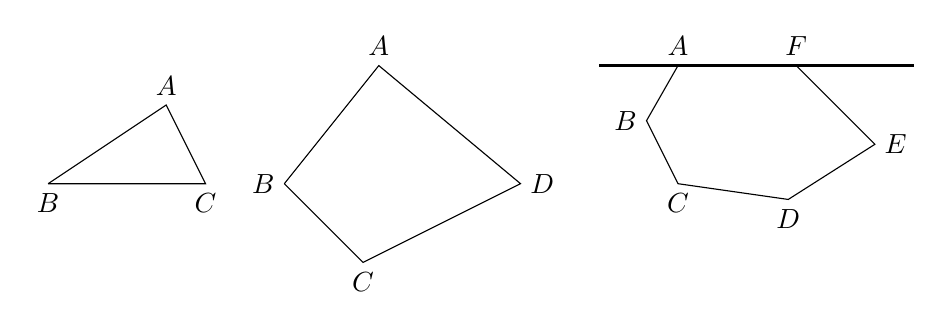
\begin{tikzpicture}
\begin{scope}
\draw(0,0)node[below]{$B$}--(2,0)node[below]{$C$}--(1.5,1)node[above]{$A$}--(0,0);
\end{scope}
\begin{scope}[xshift=3cm]
\draw (0,0)node[left]{$B$}--(1,-1)node[below]{$C$}--(3,0)node[right]{$D$}--(1.2,1.5)node[above]{$A$}--(0,0);
\end{scope}
\begin{scope}[xshift=8cm, yshift=1.5cm]
\draw (0,0)node[above]{$A$}--(1.5,0)node[above]{$F$}--(2.5,-1)node[right]{$E$}--(1.4,-1.7)node[below]{$D$}--(0,-1.5)node[below]{$C$}--(-.4,-.7)node[left]{$B$}--(0,0);
\draw[thick](-1,0)--(3,0);
\end{scope}        
    \end{tikzpicture}
    \caption{}
\end{figure}

\begin{figure}[htp]
    \centering
\begin{tikzpicture}
\draw[dashed](-2,0)--(2,0);
\draw (-.5,0)--(0.2,0)--(.3,-1)--(.7,1.8)--(-.5,0);
\end{tikzpicture}
    \caption{}
\end{figure}

\begin{blk}{定义}
两个能够完全叠合的三角形叫做\textbf{全等三角形}。两
个全等三角形完全叠合时,互相叠合的顶点叫做\textbf{对应点},互
相叠合的边叫做\textbf{对应边},互相叠合的角叫做\textbf{对应角}。因此,
\textbf{全等三角形的对应边相等,对应角相等}。
\end{blk}
 
怎样判定两个三角形全等呢?
\begin{enumerate}
\item 有两边和它们的夹角对应相等的两个三角形全
等。(SAS)
\item 有两角和它们的夹边对应相等的两个三角形全
等。(ASA)
\item 有三边对应相等的两个三角形全等。(SSS)
\end{enumerate}

利用三角形的全等,是判断两条线段或两个角相等的一
种基本方法。

\begin{example}
    在图3.3中,已知$\overline{AB}=\overline{AC}$, $\angle B=\angle C$
    
    求证:$\overline{BD}=\overline{CE}$.
\end{example}



\begin{analyze}
    要证$\overline{BD}=\overline{CE}$, 从图
上看$\overline{BD}$, $\overline{CE}$分别是$\triangle ABD$和
$\triangle ACE$的边,因此只要证明
$\triangle ACE \cong \triangle ABD$就行了,由已
知条件$\overline{AC}=\overline{AB}$, $\angle B=\angle C$而
$\angle A$是公共角,所以$\triangle ABD$与
$\triangle ACE$全等是很显然的。
\end{analyze}

\begin{proof}
在$\triangle ABD$与$\triangle ACE$中,

$\because\quad \overline{AB}=\overline{AC},\quad \angle B=\angle C$(已知)。

而$\angle A=\angle A$(公共角),

$\therefore\quad \triangle ABD\cong \triangle ACE$ (ASA).

$\therefore\quad \overline{BD}=\overline{CE}$ (全等三角形的对应边相等)。
\end{proof}    


\begin{figure}[htp]\centering
    \begin{minipage}[t]{0.48\textwidth}
    \centering
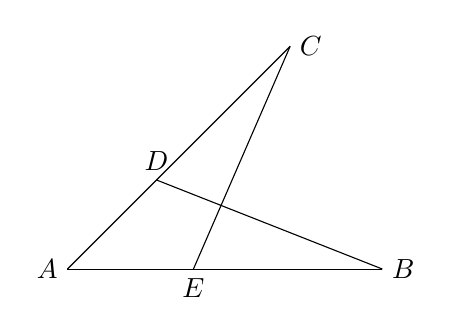
\begin{tikzpicture}[>=latex, scale=.8]
       \draw (0,0)node[left]{$A$}--(5,0)node[right]{$B$};
\draw (0,0)--(45:5)node[right]{$C$};
\draw (2,0)node[below]{$E$}--(45:5);
\draw (45:2)node[above]{$D$}--(5,0);
    \end{tikzpicture}
    \caption{}
    \end{minipage}
    \begin{minipage}[t]{0.48\textwidth}
    \centering
    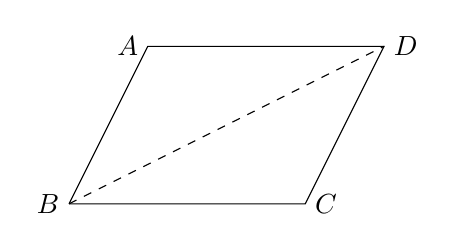
\begin{tikzpicture}[>=latex, scale=1]
        \draw (0,0)node[left]{$B$}--(3,0)node[right]{$C$}--(4,2)node[right]{$D$}--(1,2)node[left]{$A$}--(0,0);
        \draw[dashed](0,0)--(4,2);   
    \end{tikzpicture}
    \caption{}
    \end{minipage}
    \end{figure}


\begin{example}
    已知:在四边形$ABCD$中,$\overline{AD}=\overline{BC}$,
$\overline{AB}=\overline{CD}$(图3.4)。

求证:$\angle A=\angle C$。
\end{example}

\begin{analyze}
    要证明$\angle A=\angle C$, 
需要把四边形$ABCD$分成两个三
角形,为此,连结$B$、$D$. 这叫
做添\textbf{辅助线}。这样只需证
$\triangle ABD\cong \triangle CDB$就行了。
\end{analyze}

\begin{proof}
连结$B$、$D$, 在$\triangle ABD$与$\triangle CDB$中,

$\because\quad \overline{AD}=\overline{BC},\quad \overline{AB}=\overline{CD}$ (已知)

又$\because\quad \overline{BD}=\overline{BD}$ (公共边)

$\therefore\quad \triangle ABD\cong \triangle CDB$ (SSS)

$\therefore\quad \angle A=\angle C$(全等三角形的对应角相等)。
\end{proof}    

\begin{example}
在图3.5中,已知:$\overline{AB}=\overline{CD}$, $\angle B=\angle CDF$, $\overline{BD}=\overline{EF}$.

求证:$\overline{AE}=\overline{CF}$.
\end{example}

\begin{analyze}
    要证$\overline{AE}=\overline{CF}$, 只需证$\triangle ABE\cong \triangle CDF$. 由已
知,$\overline{AB}=\overline{CD}$, $\angle B=\angle CDF$, $\overline{BD}=\overline{EF}$, 虽然不能马上说
$\triangle ABE$和$\triangle CDF$全等,但只要注意到$\overline{BD}+\overline{DE}=\overline{DE}+\overline{EF}$, 
即$\overline{EB}=\overline{DF}$就行了。
\end{analyze}

\begin{proof}
    在图3-5中,$\because\quad \overline{BD}=\overline{EF}$ 已知

$\therefore\quad \overline{BD}+\overline{DE}=\overline{DE}+\overline{EF}$ (等量加等量和相等)。即:
\[\overline{BE}=\overline{DF}\]
又$\because\quad \overline{AB}=\overline{CD},\; \angle B =\angle CDF$ 已知

$\therefore\quad \triangle ABE\cong \triangle CDF$ (SAS).

$\therefore\quad \overline{AE}=\overline{CF}$ (全等三角形的对应边相等)。
\end{proof}

\begin{figure}[htp]\centering
    \begin{minipage}[t]{0.48\textwidth}
    \centering
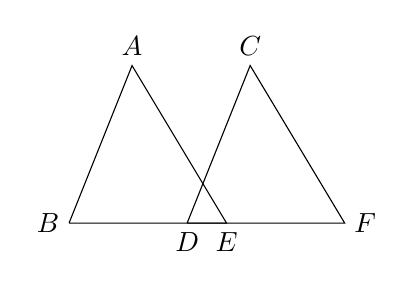
\begin{tikzpicture}[>=latex, scale=1]
       \draw(0,0)node[left]{$B$}--(2,0)node[below]{$E$}--(.8,2)node[above]{$A$}--(0,0);
\draw(1.5,0)node[below]{$D$}--(3.5,0)node[right]{$F$}--(2.3,2)node[above]{$C$}--(1.5,0);
    \end{tikzpicture}
    \caption{ }
    \end{minipage}
    \begin{minipage}[t]{0.48\textwidth}
    \centering
    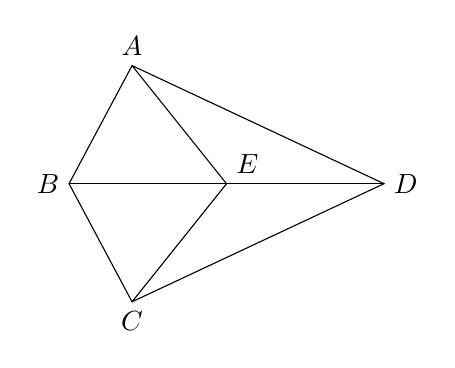
\begin{tikzpicture}[>=latex, xscale=.8]
      \draw(0,0)node[left]{$B$}--(5,0)node[right]{$D$};
      \draw(1,1.5)node[above]{$A$}--(2.5,0)node[above right]{$E$}--(1,-1.5)node[below]{$C$}--(0,0)--(1,1.5)--(5,0)--(1,-1.5);
    \end{tikzpicture}
    \caption{ }
    \end{minipage}
    \end{figure}

\begin{example}
    在图3.6中,已知:$\overline{AB}=\overline{BC}$, $\overline{AD}=\overline{CD}$, $E$点在$BD$上。

求证:$\overline{AE}=\overline{CE}$.
\end{example}

\begin{analyze}
    要证$\overline{AE}=\overline{CE}$, 只需证明$\triangle ABE\cong \triangle CBE$, 或者证明$\triangle ADE\cong \triangle CDE$, 假定我们证明$\triangle ABE\cong \triangle CBE$,
    已知$\overline{AB}=\overline{BC}$, $\overline{BE}=\overline{BE}$, 因此只需证明$\angle ABD=\angle CBD$;
    要证$\angle ABD=\angle CBD$, 只需证明$\triangle ABD\cong\triangle CBD$.
\end{analyze}

\begin{proof}
    在$\triangle ABD$与$\triangle CBD$中,

    $\because\quad \overline{AB}=\overline{CB},\quad \overline{AD}=\overline{CD}$ (已知)   $\overline{BD}=\overline{BD}$(公共边)

    $\therefore\quad \triangle ABD\cong \triangle CBD$ (SSS).

    $\therefore\quad \angle ABD=\angle CBD$ (全等三角形的对应角相等)

$\because\quad     \overline{AB}=\overline{BC}$ (已知) 
    $\overline{BE}=\overline{BE}$ (公共边)

$\therefore\quad \triangle ABE\cong \triangle CBE$ (SAS).

$\therefore\quad \overline{AE}=\overline{CE}$ (全等三角形的对应边相等)。
\end{proof}

    利用三角形全等,来证明两条线段或两个角相等,关键
    在于找出能够全等的三角形,并且使要证明的线段和角恰好
    成为它们的对应边和对应角。为了找出全等的三角形,必要
    时需要添加辅助线。  

\begin{ex}
\begin{enumerate}
    \item 已知:在四边形$ABCD$中,$AC$平分$\angle BAD$, $\overline{AB}=\overline{AD}$.
    
    求证:$\angle ACB=\angle ACD$.
    \item 已知:如图,$\overline{AC}$、$\overline{BD}$交于$O$点,    且$\overline{AO}=\overline{OC}$、$\overline{BO}=\overline{OD}$.
    
    求证:$\overline{AB}=\overline{CD}$.


\item 已知:如图,$\angle 1=\angle 4$, $\angle 2=\angle 3$.
求证:$\overline{AB}=\overline{CD}$.
\item 已知:如图,$\angle 1=\angle 2$, $\angle 3=\angle 4$, $\overline{AB}=\overline{AD}$. 

求证:$\overline{AE}=\overline{AC}$, $\angle E=\angle C$.

\item 已知:如图,$\angle 1=\angle 2$, $\angle 3=\angle 4$,
求证:$\overline{AC}=\overline{BD}$.
\item 已知:如图,在四边形$ABCD$中,$\overline{AB}=\overline{BC}$, $\overline{AD}=\overline{CD}$.

求证:$\angle A=\angle C$.
\item 已知:如图,$\overline{AD}=\overline{BE}$, $\overline{AE}=\overline{BD}$, AC、BC是直线。

求证:$\angle CDB=\angle CEA$.
\item 已知:如图,$\overline{AB}=\overline{CD}$, E、F分别是$\overline{AB}$、$\overline{CD}$的中点,
并且$\overline{BF}=\overline{CE}$.

求证:$\angle EBC=\angle FCB$, $\angle FBC=\angle ECB$.

\item 已知:如图,在四边形$ABCD$中,$\overline{AB}=\overline{CD}$, $\overline{AD}=\overline{BC}$, $\overline{EF}$过$\overline{BD}$的中点$O$. 

求证:$\overline{OE}=\overline{OF}$.
\end{enumerate}
\end{ex}

\begin{figure}[htp]\centering
    \begin{minipage}[t]{0.48\textwidth}
    \centering
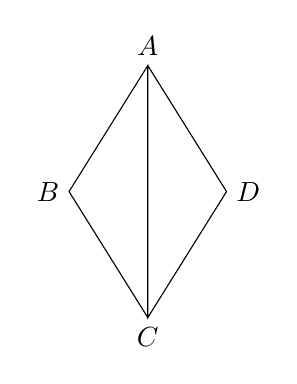
\begin{tikzpicture}[>=latex, yscale=.8]
       \draw(0,2)node[above]{$A$}--(1,0)node[right]{$D$}--(0,-2)node[below]{$C$}--(0,2)--(-1,0)node[left]{$B$}--(0,-2);
    \end{tikzpicture}
    \caption*{第1题}
    \end{minipage}
    \begin{minipage}[t]{0.48\textwidth}
    \centering
    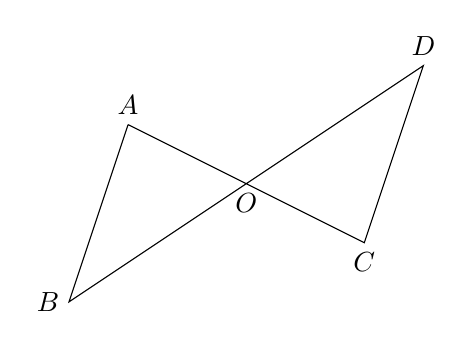
\begin{tikzpicture}[>=latex, scale=1.5]
      \draw(-1,.5)node[above]{$A$}--(1,-.5)node[below]{$C$}--(1.5,1)node[above]{$D$}--(-1.5,-1)node[left]{$B$}--(-1,.5);
      \node at (0,0)[below]{$O$};
    \end{tikzpicture}
    \caption*{第2题}
    \end{minipage}
    \end{figure}

\begin{figure}[htp]\centering
    \begin{minipage}[t]{0.48\textwidth}
    \centering
\begin{tikzpicture}[>=latex, scale=1.3]
\tkzDefPoints{1/2/A, 0/0/B, 3/0/C, 4/2/D}
\tkzDrawPolygon(A,B,C)
\tkzDrawPolygon(A,D,C)
\tkzMarkAngle[mark=none, size=.35](B,A,C)  
\tkzLabelAngle[pos=.5](B,A,C) {2}
\tkzMarkAngle[mark=none, size=.5](C,A,D)  
\tkzLabelAngle[pos=.7](C,A,D) {1}
 \tkzLabelAngle[pos=.75](A,C,B) {4}
\tkzMarkAngle[mark=none, size=.5](D,C,A)  
\tkzLabelAngle[pos=.25](D,C,A) {3}
\tkzMarkAngle[mark=none, size=.6](A,C,B) 
\tkzLabelPoints[left](A,B)
\tkzLabelPoints[right](C,D)
    \end{tikzpicture}
    \caption*{第3题}
    \end{minipage}
    \begin{minipage}[t]{0.48\textwidth}
    \centering
    \begin{tikzpicture}[>=latex, scale=1.3]
        \tkzDefPoint(0,0){A}
        \tkzDefPoint(-90:2){B}
        \tkzDefPoint(-60:2){D}
        \tkzDefPoint(0:2.75){E}
        \tkzDefPoint(-30:2.75){C}
        \tkzLabelPoints[left](A,B)
        \tkzDrawPolygon(A,B,D)
\tkzDrawLines[add=0 and 1.38](B,D) %\tkzGetPoint{C}
\draw (D)--(E)--(A)--(C);
\tkzLabelPoints[right](C,E)
\tkzLabelPoints[below](D)
\tkzMarkAngles[mark=none, size=.44](C,A,E B,A,D C,B,A E,D,A)  
\tkzLabelAngle[pos=.65](C,A,E) {2}
\tkzLabelAngle[pos=.65](B,A,D) {1}
\tkzLabelAngle[pos=.6](C,B,A) {3}
\tkzLabelAngle[pos=.6](E,D,A) {4}


    \end{tikzpicture}
    \caption*{第4题}
    \end{minipage}
    \end{figure}



\begin{figure}[htp]\centering
    \begin{minipage}[t]{0.48\textwidth}
    \centering
\begin{tikzpicture}[>=latex, scale=1]
\tkzDefPoints{-1/2/A, 1/2/D, -2/-1/B, 2/-1/C}
\tkzDrawPolygon(A,C,D) \tkzDrawPolygon(A,B,D)
\tkzLabelPoints[left](A,B)
\tkzLabelPoints[right](C,D)
\tkzMarkAngles[mark=none, size=.6](C,A,D A,D,B) 
\tkzMarkAngles[mark=none, size=.5](B,A,C B,D,C) 
\tkzLabelAngle[pos=.7](C,A,D) {1}
\tkzLabelAngle[pos=.7](A,D,B) {2}
\tkzLabelAngle[pos=.65](B,A,C) {3}
\tkzLabelAngle[pos=.65](B,D,C) {4}



    \end{tikzpicture}
    \caption*{第5题}
    \end{minipage}
    \begin{minipage}[t]{0.48\textwidth}
    \centering
    \begin{tikzpicture}[>=latex, scale=1.3]
        \tkzDefPoints{-1/0/B, 2/0/D, 1/1/A, 1/-1/C, 0/0/O} 
        \tkzDrawPolygon(A,B,C,D)
        \tkzAutoLabelPoints[center=O](A,B,C,D)

    \end{tikzpicture}
    \caption*{第6题}
    \end{minipage}
    \end{figure}




\begin{figure}[htp]\centering
    \begin{minipage}[t]{0.48\textwidth}
    \centering
\begin{tikzpicture}[>=latex, scale=1]
    \tkzDefPoints{-1.5/0/A, 1.5/0/B, 0/3/C, 0/1.5/O}  
    \tkzDefMidPoint(A,C)\tkzGetPoint{D}
    \tkzDefMidPoint(B,C)\tkzGetPoint{E}    
    \tkzDrawPolygon(A,B,C)
    \draw(B)--(D)node[left]{$D$};
    \draw (A)--(E)node[right]{$E$};
    \tkzAutoLabelPoints[center=O](A,B,C)
    \end{tikzpicture}
    \caption*{第7题}
    \end{minipage}
    \begin{minipage}[t]{0.48\textwidth}
    \centering
    \begin{tikzpicture}[>=latex, scale=.8]
        \tkzDefPoints{-2.5/0/B, 2.5/0/C, -1.5/3/A, 1.5/3/D,  0/1.5/O}  
        \tkzDefMidPoint(A,B)\tkzGetPoint{E}
        \tkzDefMidPoint(D,C)\tkzGetPoint{F}    
        \tkzDrawPolygon(A,B,C,D)
        \draw(B)--(F)node[right]{$F$};
        \draw (C)--(E)node[left]{$E$};
        \tkzAutoLabelPoints[center=O](A,B,C,D)
    \end{tikzpicture}
    \caption*{第8题}
    \end{minipage}
    \end{figure}


\begin{figure}[htp]\centering
    \begin{minipage}[t]{0.48\textwidth}
    \centering
\begin{tikzpicture}[>=latex, scale=.8]
    \tkzDefPoints{-2.5/0/B, 2.5/0/C, -1.5/3/A, 3.5/3/D}  
    \tkzDefMidPoint(D,B)\tkzGetPoint{O}
    \tkzDrawPolygon(A,B,C,D)
\draw (0,3)node[above]{$E$}--(1,0)node[below]{$F$};
\tkzAutoLabelPoints[center=O](A,B,C,D)
\draw(B)--(D);
\node at (O)[right]{$O$};

    \end{tikzpicture}
    \caption*{第9题}
    \end{minipage}
    \begin{minipage}[t]{0.48\textwidth}
    \centering
    \begin{tikzpicture}[>=latex, scale=1]
\tkzDefPoints{-1.5/0/B, 1.5/0/C, 0/3/A, 0/1.5/O}
\tkzDrawPolygon(A,B,C)
\tkzAutoLabelPoints[center=O](A,B,C)
\tkzMarkAngles[mark=none, size=.5](C,B,A A,C,B B,A,C) 
\node at (0,-.25){底};\node at (0,2.25){顶角};
\node at (-1,1.5){腰};\node at (1,1.5){腰};
\node(A) at (0,.25){底角};
\draw[<-](-1,.25)--(A);
\draw[<-](1,.25)--(A);
    \end{tikzpicture}
    \caption{}
    \end{minipage}
    \end{figure}

\subsection{等腰三角形}

\begin{blk}{定义}
    有两条边相等的三角形叫做\textbf{等腰三角形}。相等的两边
叫做\textbf{腰},另外的一边叫做\textbf{底},腰和底的夹角叫做\textbf{底角},两腰的夹
角叫\textbf{顶角},如图3.7所示。
\end{blk}

\begin{blk}{定义}
    三角形的一个角的平分线与对边相交,这个角的
    顶点和交点之间的线段叫做\textbf{三角形的角的平分线}。在图
    3.8(1)中,$\overline{AF}$平分$\angle A$, 交对边于$F$点,$\overline{AF}$就是$\triangle ABC$
    的$\angle A$的平分线。  

    连结三角形一个顶点和它的对边中点的线段叫做\textbf{三角形
的中线}。在图3.8(2)中,$E$点是$\overline{BC}$的中点,$\overline{AF}$就是$\triangle ABC$的$\overline{BC}$边上的中线。

从三角形一个顶点到它的对边所在直线作垂线,顶点和
垂足之间的线段叫做\textbf{三角形的高线}(简称\textbf{高})。在图3.8(3)
中,$\overline{AD}\bot$直线$BC$, $D$是垂足,$\overline{AD}$就是$\triangle ABC$的$\overline{BC}$边上
的高线。
\end{blk}

\begin{figure}[htp]
    \centering
\begin{tikzpicture}[scale=.8]
\begin{scope}
\tkzDefPoints{0/0/B, 3.6/0/F, 5.5/0/C, 4.5/3/A}
\tkzDrawPolygon(A,B,C)
\draw(A)--(F);
\tkzMarkAngles[mark=none, size=.5](B,A,F) 
\tkzMarkAngles[mark=none, size=.6](F,A,C)
\tkzLabelAngle[pos=.7](B,A,F) {1}
\tkzLabelAngle[pos=.75](F,A,C) {2}

\tkzLabelPoints[below](C, F, B)
\tkzLabelPoint(A){$A$}
\node at (2.7,-1){(1)};
\end{scope}
\begin{scope}[xshift=7cm]
    \tkzDefPoints{0/0/B, 2/0/E, 4/0/C, 4.5/3/A}
    \tkzDrawPolygon(A,B,C)
    \tkzLabelPoints[below](C, E, B)
    \tkzLabelPoint(A){$A$}
    \draw(E)--(A);
    \node at (2.2,-1){(2)};
\end{scope}    
\begin{scope}[yshift=-5cm]
\draw (0,0)node[below]{$B$}--(5.5,0)node[below]{$C$}--(4.5,3)node[above]{$A$}--(0,0);
\tkzDefPoints{4.5/3/A1, 4.5/0/D1, 5.5/0/C1}
\tkzMarkRightAngle(A1,D1,C1)
\draw(4.5,3)--(4.5,0)node[below]{$D$};
\draw(11,3)--(11,0)node[below]{$D$};
\draw[dashed](9,0)--(12,0);
\draw (7,0)node[below]{$B$}--(9.5,0)node[below]{$C$}--(11,3)node[above]{$A$}--(7,0);
\tkzDefPoints{11/3/A2, 11/0/D2, 9.5/0/C2}
\tkzMarkRightAngle(A2,D2,C2)
\node at (6,-1){(3)};
\end{scope}
\end{tikzpicture}
    \caption{}
\end{figure}

三角形的高线、中线、角平分线,一般是指一条线段,
但有时当我们不考虑其长度时,也把它们分别所在的直线叫
做三角形的高线、中线、角的平分线。


\begin{blk}
    {等腰三角形性质定理} 等腰三角形底角相等。
\end{blk}

已知:在$\triangle ABC$中;$AB=AC$.
求证:$\angle B=\angle C$.

\begin{figure}[htp]
    \centering
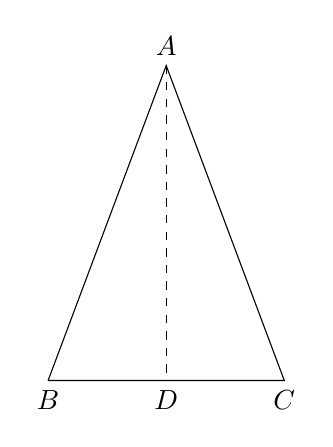
\begin{tikzpicture}
\draw (0,0)node[below]{$B$}--(3,0)node[below]{$C$}--(1.5,4)node[above]{$A$}--(0,0);
\draw[dashed](1.5,4)--(1.5,0)node[below]{$D$};
\end{tikzpicture}
    \caption{}
\end{figure}
\begin{proof}
    作$\angle BAC$的平分线$\overline{AD}$
(图3.9),在$\triangle ABD$和$\triangle ACD$
中

$\because\quad AB=AC$ (已知),$\overline{AD}=\overline{AD}$(公共边),$\angle BAD=\angle CAD$(角平分线定义)

$\therefore\quad \triangle ABD≤\triangle ACD$(SAS)

$\therefore\quad \angle B=\angle C$(全等三角形的对应角相等)。
\end{proof}


由于 $\overline{BD}=\overline{DC},\; \angle BDA=\angle CDA=90^{\circ}$

因此 $AD$平分$\overline{BC}$, 且$AD\bot BC$.

\begin{blk}{推论 }
    等腰三角形顶角的平分线垂直、平分底边。
\end{blk}

也就是说,等腰三角形的顶角平分线也是底边上的高线
和中线。(\textbf{三线合一})

\begin{blk}
    {等腰三角形的判定定理} 有两个角相等的三角形是等腰
三角形。
\end{blk}

已知:在$\triangle ABC$中,$\angle B=\angle C$(图3.10)。
求证:$\overline{AB}=\overline{AC}$.

\begin{figure}[htp]
    \centering
\begin{tikzpicture}
\draw(0,0)node[left]{$B$}--(2,0)node[right]{$C$}--(1,2)node[above]{$A$}--(0,0);
\draw(4,2)node[left]{$B'$}--(6,2)node[right]{$C'$}--(5,0)node[below]{$A'$}--(4,2);
\end{tikzpicture}
    \caption{}
\end{figure}


\begin{proof}
    根据翻转公理,我们可以把$\triangle ABC$翻转过来,
    设顶点$A$、$B$、$C$成为$A'$、$B'$、$C'$.
    
    $\because\quad \angle B=\angle C=\angle C',\quad \angle C=\angle B=\angle B'$

    又:$\because\quad \overline{BC}=\overline{C'B'}$

    $\therefore\quad \triangle ABC\cong \triangle A'C'B'$(ASA)

    $\therefore\quad \overline{AB}=\overline{A'C'}$(全等三角形的对应边相等)。

由于$\overline{AC}=\overline{A'C'}$,$\therefore\quad \overline{AB}=\overline{AC}$(等量代换)
\end{proof}

用逻辑语句说:等腰三角形的判定定理是其性质定理的
逆定理。这两个定理我们用“充要”条件可合写成一个定理:

\begin{blk}{}
   一个三角形是等腰三角形的充要条件是这个三角形有两
个角相等。
\end{blk}


\begin{blk}{定义}
    三条边都相等的三角形叫做\textbf{等边三角形},也叫做
    \textbf{正三角形}。
\end{blk}


同学们自己证明下面等边三角形的性质定理和判定定
理。

\begin{blk}{}
    \begin{itemize}
        \item 等边三角形的三内角相等。
        \item   三内角相等的三角形是等边三角形。
    \end{itemize}
\end{blk}

由等腰三角形及等边三角形的性质定理和判定定理可
知,在一个三角形中,由边的相等可以推知角的相等,反过
来由角的相等也可推知边的相等。下面举例说明它们在证题
中的应用。

\begin{example}
已知:在图3.11中,$\overline{AB}=\overline{EB}$, 
$\overline{AC}=\overline{DC}$, 
ADB、AEC是直线。

求证:$\angle ADC=\angle AEB$.
\end{example}

\begin{analyze}
    要证$\angle ADC=\angle AEB$,
只需证明$\angle ADC=\angle A$, $\angle AEB=\angle A$; 要证明
$\angle ADC=\angle A$, $\angle AEB=\angle A$, 只要知道$\overline{AC}=\overline{DC}$, 
$\overline{AB}=\overline{BE}$就行了。
\end{analyze}

\begin{proof}
    在$\triangle BAE$中,
$\because\quad \overline{AB}=\overline{EB}$(已知),

$\therefore\quad \angle AEB=\angle A$(等腰三角形的底角相等)。

在$\triangle CAD$中,
$\because\quad \overline{AD}=\overline{DC}$(已知),

$\therefore\quad \angle ADC=\angle A$(等腰三角形的底角相等)。

$\therefore\quad \angle ADC=\angle AEB$ (等量代换)。
\end{proof}

\begin{figure}[htp]\centering
    \begin{minipage}[t]{0.48\textwidth}
    \centering
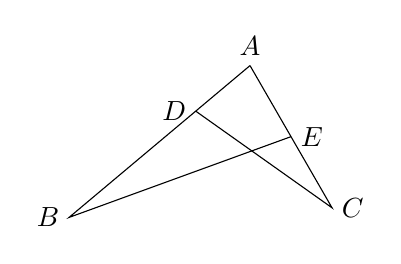
\begin{tikzpicture}[>=latex, scale=1]
\draw(40:3)node[above]{$A$}--(0,0)node[left]{$B$}--(20:3)node[right]{$E$};
\draw(40:3)--(3.34,0.122)node[right]{$C$}--(40:2.1)node[left]{$D$};
    \end{tikzpicture}
    \caption{}
    \end{minipage}
    \begin{minipage}[t]{0.48\textwidth}
    \centering
    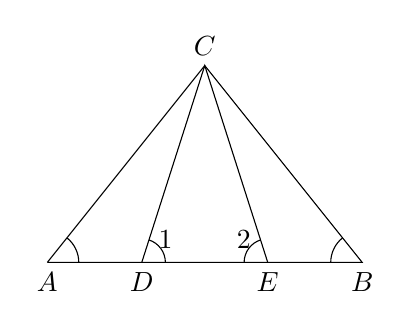
\begin{tikzpicture}[>=latex, scale=1]
\draw(-2,0)node[below]{$A$}--(0,2.5)node[above]{$C$}--(2,0)node[below]{$B$}--(-2,0);
\draw(.8,0)node[below]{$E$}--(0,2.5)--(-.8,0)node[below]{$D$};
\draw (-2+.4,0) arc (0:51.34:.4);
\draw (2-.4,0) arc (180:180-51.34:.4);
\draw (-.8+.3,0) arc (0:72.3:.3)node[right]{1};
\draw (.8-.3,0) arc (180:180-72.3:.3)node[left]{2};
    \end{tikzpicture}
    \caption{}
    \end{minipage}
    \end{figure}


\begin{example}
    如图3.12, 
己知:$\overline{AC}=\overline{BC}$, $\overline{AE}=\overline{DB}$. 

求证:$\overline{CD}=\overline{CE}$.
\end{example}

\begin{analyze}
    在$\triangle CDE$中,若要证$\overline{CD}=\overline{CE}$,
   只要证$\angle 1=\angle 2$即可, $\angle 1$和$\angle 2$分别在$\triangle BCD$与$\triangle ACE$中,如能证明$\triangle BCD\cong \triangle ACE$, 即可证明$\angle 1=\angle 2$.
\end{analyze}

\begin{solution}
在$\triangle ACE$与$\triangle BCD$中,

$\because\quad \overline{AC}=\overline{BC},\quad \overline{AE}=\overline{BD}$ (已知)

$\therefore\quad \angle A=\angle B$(等腰三角形两底角相等),

$\therefore\quad \triangle ACE\cong \triangle BCD$(SAS)

$\therefore\quad \angle 2=\angle 1$(全等三角形的对应角相等),

$\therefore\quad \triangle CDE$ 是等腰三角形(有两角相等的三角形是等腰三角形)。

$\therefore\quad \overline{CD}=\overline{CE}$
\end{solution}

\begin{ex}
\begin{enumerate}
    \item 画出$\triangle ABC$和$\triangle DEF$的三条边上的高线。
    \item 画一个三角形$ABC$, 然后画出$\triangle ABC$三个内角的平分线。
    \item 画一个三角形$DEF$, 然后画出$\triangle DEF$三边上的中线。
    \item 证明:全等三角形的对应角的平分线相等。
    \item 证明:全等三角形对应边上的中线相等。
    \item 已知:$A=\{\text{等腰三角形}\}$,$B=\{\text{两内角相等的三角
    形}\}$,指出集合$A$与集合$B$的关系。
    \item 若$\overline{AC}=\overline{BC},\quad \angle DCA=\angle ECB$, 则$\overline{CD}=\overline{CE}$.
    \item 若$\overline{AC}=\overline{BC},\quad \angle 1=\angle 2$, 则$\overline{AE}=\overline{BD}$.
    \item 若$\overline{AC}=\overline{BC}$, $\overline{AD}$、$\overline{BE}$分别是$\angle A$和$\angle B$的平分线,
    则$\overline{AD}=\overline{BE}$.
    \item 若$\overline{AC}=\overline{BC},\quad \overline{AD}=\overline{BE}$, $DE$是直线,则$\triangle DEC$是等腰
三角形。
\item 若$\overline{AC}=\overline{BC},\quad \angle ACD=\angle BCE$, $DE$是直线,则$\triangle DEC$
是等腰三角形。
\item 在等边$\triangle ABC$的三边上,分别取$D$、$E$、$F$(如图),
使$\overline{AD}=\overline{BE}=\overline{CF}$, 则$\triangle DEF$是等边三角形。
\item 设$\overline{DE}=\overline{EF}=\overline{FD}$, $\angle AFD=\angle BDE=\angle CEF$, 
则$\triangle ABC$是等边三角形。
\end{enumerate}
\end{ex}

\begin{figure}[htp]
    \centering
\begin{tikzpicture}
\begin{scope}
    \draw(0,0)node[below]{$B$}--(1.5,.2)node[below]{$C$}--(2,2)node[above]{$A$}--(0,0);
\end{scope}
\begin{scope}[xshift=5cm]
    \draw(0,0)node[below]{$E$}--(2,0)node[below]{$F$}--(.7,1.5)node[above]{$D$}--(0,0);
\end{scope}
\end{tikzpicture}
    \caption*{第1题}
\end{figure}

\begin{figure}[htp]\centering
    \begin{minipage}[t]{0.48\textwidth}
    \centering
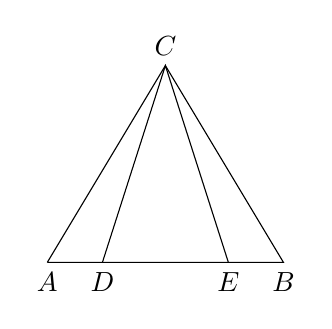
\begin{tikzpicture}[>=latex, scale=1]
\draw(-1.5,0)node[below]{$A$}--(0,2.5)node[above]{$C$}--(1.5,0)node[below]{$B$}--(-1.5,0);
\draw(.8,0)node[below]{$E$}--(0,2.5)--(-.8,0)node[below]{$D$};
    \end{tikzpicture}
    \caption*{第7题}
    \end{minipage}
    \begin{minipage}[t]{0.48\textwidth}
    \centering
    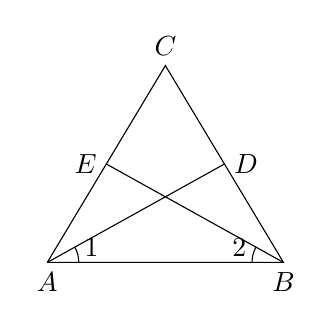
\begin{tikzpicture}[>=latex, scale=1]
\draw(-1.5,0)node[below]{$A$}--(0,2.5)node[above]{$C$}--(1.5,0)node[below]{$B$}--(-1.5,0);
\draw(-.75,1.25)node[left]{$E$}--(1.5,0);
\draw(.75,1.25)node[right]{$D$}--(-1.5,0);
\draw(-1.5+.4,0) arc (0:29:.4)node[right]{1};
\draw(1.5-.4,0) arc (180:180-29:.4)node[left]{2};
    \end{tikzpicture}
    \caption*{第8--9题}
    \end{minipage}
    \end{figure}

\begin{figure}[htp]\centering
    \begin{minipage}[t]{0.48\textwidth}
    \centering
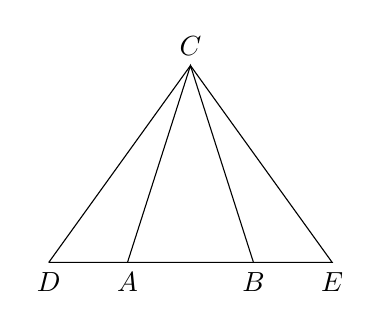
\begin{tikzpicture}[>=latex, scale=1]
    \draw(-1.8,0)node[below]{$D$}--(0,2.5)node[above]{$C$}--(1.8,0)node[below]{$E$}--(-1.8,0);
    \draw(.8,0)node[below]{$B$}--(0,2.5)--(-.8,0)node[below]{$A$};
    \end{tikzpicture}
    \caption*{第10--11题}
    \end{minipage}
    \begin{minipage}[t]{0.48\textwidth}
    \centering
    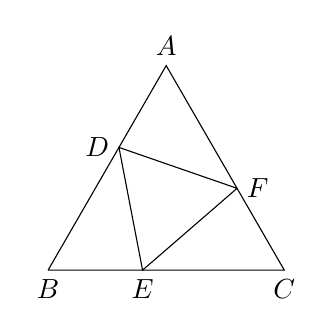
\begin{tikzpicture}[>=latex, scale=1]
\draw(-120:3)node[below]{$B$} --(0,0)node[above]{$A$}--(-60:3)node[below]{$C$}-- (-120:3) ;
\draw(-60:1.8)node[right]{$F$}--(-120:1.2)node[left]{$D$}--(-.3,-1.5*1.732)node[below]{$E$}--(-60:1.8);
    \end{tikzpicture}
    \caption*{第12--13题}
    \end{minipage}
    \end{figure}

\subsection{轴对称图形}
\begin{blk}{定义}
    在平面上有两个图形$F$和$F'$, 如果平面沿着某
条直线$\ell$折叠起来,$F$和$F'$叠合,就称$F$和$F'$关于$\ell$成\textbf{轴对
称}。(也称$F$和$F'$是以$\ell$为轴的\textbf{对称形})。$F$和$F'$上互相叠合
的点叫做\textbf{对称点},$\ell$叫做\textbf{对称轴}。
\end{blk}

在图3.13(1)中,平面上的$\triangle ABC$和$\triangle A'B'C'$关于直
线$\ell$成轴对称;$A$与$A'$、$B$与$B'$、$C$与$C'$都是对称点。

\begin{figure}[htp]
    \centering
\begin{tikzpicture}
\begin{scope}
    \draw(0,-.5)--(0,4)node[above]{$\ell$};
    \node at (0,-1){(1)};

\draw(-1.8,2)node[above]{$B$}--(-.4,3)node[above]{$A$}--(-1.4,0.5)node[below]{$C$}--(-1.8,2);
\draw(1.8,2)node[above]{$B'$}--(.4,3)node[above]{$A'$}--(1.4,0.5)node[below]{$C'$}--(1.8,2);

\end{scope}
\begin{scope}[xshift=6.5cm]
    \draw(0,-.5)--(0,4)node[above]{$\ell$};
\draw(-2,0)node[below]{$B$}--(2,0)node[below]{$C$}--(0,3)node[right]{$A$}--(-2,0);
\draw (0,0) rectangle (.2,.2);
\node at (0,-1){(2)};
\end{scope}
\end{tikzpicture}
    \caption{}
\end{figure}

\begin{blk}{推论}
     两个图形如果关于某直线成轴对称,那么这两个
图形是全等形。
\end{blk}

\begin{blk}{定义}
    如果一个图形可以分成两部分,这两部分关于某
一直线成轴对称,就把这个图形称为\textbf{轴对称形}。
\end{blk}

显然,等腰三角形关于它的顶角平分线成轴对称图形
(图3.13(2))。轴对称形在实际中应用非常广泛,图3.14中
的图形,都是轴对称形。
\begin{figure}[htp]
    \centering
\includegraphics[scale=.6]{fig/3-14.png}
    \caption{}
\end{figure}

轴对称图形有什么性质呢?这就要研究一下对称轴和对
称点的关系。

在图3.15中,设$A$与$A'$是关于直线$\ell$的轴对称点,因为
$A$、$A'$和$\ell$在同一平面内,并且$A$和$A'$在$\ell$的两侧,所以线段
$\overline{AA'}$与$\ell$必相交,设交点为$O$, 在$\ell$上取异于$O$的另一点$P$, 连
结$\overline{AP}$,$\overline{A'P}$.

由于$A$点所在的半平面沿直线$\ell$折叠过来,$A$和$A'$重合,
而$\ell$上的$P$和$O$重合于自身,所以$\overline{AP}=\overline{A'P}$, $\angle APO=\angle A'PO$, $\triangle PAA'$是等腰三角形,直线$\ell$是顶角的平分线,
所以$\ell$垂直平分底边$\overline{AA'}$.

由此得出轴对称图形的重要性质:
\begin{enumerate}
\item 对称轴上的任一点,与每一双对称点的距离相等。
\item 对称轴是每一双对称点所连线段的垂直平分线。
\end{enumerate}

在上述性质的证明中,我们所取$P$点异于$O$, 如果$P$点就
是$O$点,结论仍然一样。

由于一条线段的垂直平分线是唯一的,由性质2可知,
如果$\overline{AA'}$的垂直平分线是$\ell$, 那么$A$与$A'$是以$\ell$为轴的对称
点。

由此,我们就可以作出已知图形以某直线为轴的对称
形。

\begin{figure}[htp]\centering
    \begin{minipage}[t]{0.48\textwidth}
    \centering
\begin{tikzpicture}[>=latex, scale=.8]
    \draw(0,-.5)--(0,4)node[above]{$\ell$};
\draw(-2,0)node[below]{$A$}--(2,0)node[below]{$A'$}--(0,3)node[right]{$P$}--(-2,0);
\draw (0,0)node[below right]{$O$} rectangle (.2,.2);
    \end{tikzpicture}
    \caption{}
    \end{minipage}
    \begin{minipage}[t]{0.48\textwidth}
    \centering
    \begin{tikzpicture}[>=latex, scale=1]
\draw(0,-.5)--(0,4)node[above]{$\ell$};     
\tkzDefPoints{-1/3/A, 1/3/A', -2.5/2/B,2.5/2/B',-1.5/0/C,1.5/0/C',-.5/.8/D, .5/.8/D'}
\tkzDrawPolygon(A,B,C,D)\tkzDrawPolygon(A',B',C',D')
\foreach \x in {A,B,C,D}
{
    \draw(\x)--(\x');
}
\tkzDefPoints{0/2.1/O}
\tkzAutoLabelPoints[center=O](A,B,C,D,A',B',C',D')
\node at (0,3)[below right]{$O$};
\draw(0,3) rectangle (-.2,3+.2);
    \end{tikzpicture}
    \caption{}
    \end{minipage}
    \end{figure}



\begin{example}
已知:四边形$ABCD$及直线$\ell$. (图3.16)

求作:四边形$ABCD$以$\ell$为轴的轴对称形。

作法:
\begin{enumerate}
\item 由$A$点引$\ell$的垂线交$\ell$于$O$点,在射线$AO$上
取$OA'=AO$, 则$A'$是$A$点关于轴$\ell$的对称点。
\item 用同样的方法作点$B$、$C$、$D$关于$\ell$的对称点$B'$、
$C'$、$D'$.
\item 连结$\overline{A'B'}$, $\overline{B'C'}$, $\overline{C'D'}$, $\overline{D'A'}$, 则四边形
$A'B'C'D'$就是四边形$ABCD$以$\ell$为轴的轴对称图形。
\end{enumerate}

为什么呢?因为根据作法,如果把四边形$ABCD$和 四边
形$A'B'C'D'$所在平面,沿直线$\ell$折叠起来,则$A$与$A'$、
$B$与$B'$、$C$与$C'$、$D$与$D'$分别重合,所以四边形$ABCD$与
四边形$A'B'C'D'$完全重合,所以这两个四边形是以$\ell$为轴
的对称图形。
\end{example}

\begin{example}
    有公共底的两个等腰三角形,通过底所对的两个
顶点的直线是它们所组成图形的对称轴。

已知:在图3.17中,$BC$是等腰$\triangle ABC$与等腰$\triangle A'BC$
的公共底边。

求证:直线$AA'$是这个图形的对称轴。
\end{example}

\begin{figure}[htp]
    \centering
\begin{tikzpicture}[scale=.8]
\begin{scope}
\draw(0,-1.5)--(0,4);
\draw(-1.5,0)node[left]{$B$}--(1.5,0)node[right]{$C$}--(0,3)node[right]{$A$}--(-1.5,0)--(0,-1)node[right]{$A'$}--(1.5,0);

\end{scope}
\begin{scope}[xshift=7cm]
    \draw(0,-1)--(0,4);
\draw(-1.5,0)node[left]{$B$}--(1.5,0)node[right]{$C$}--(0,3)node[right]{$A$}--(-1.5,0)--(0,1.8)node[right]{$A'$}--(1.5,0);

\end{scope}
\end{tikzpicture}
    \caption{}
\end{figure}

\begin{proof}
$\because\quad \overline{AB}=\overline{AC},\quad \overline{A'B}=\overline{A'C}$(已知)

$\therefore\quad \angle ABC=\angle ACB,\quad 
\angle A'BC=\angle A'CB$(等腰三角形的两底角相等)。

两式相加(或相减)得:
$\angle ABA'=\angle ACA'$(等量加(或减)等量其和(或差)
相等)。

$\therefore\quad \triangle ABA'\cong \triangle ACA'$(SAS)

以$AA'$为轴折叠起来,$\triangle ABA'$与$\triangle ACA'$能够重
合,所以$AA'$是这个图形的对称轴。
\end{proof}

\begin{example}
    证明四条边相等的四边形的两条对角线互相垂直
平分,并且平分一双对角。

已知:在四边形$ABCD$中,$\overline{AB}=\overline{BC}=\overline{CD}=\overline{DA}$.
(图3.18)
\begin{figure}[htp]
    \centering
    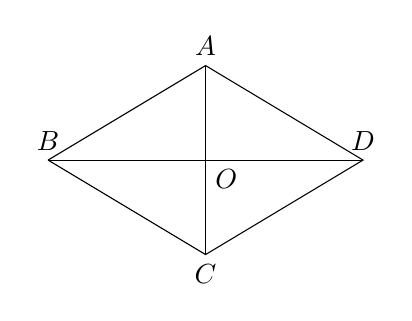
\begin{tikzpicture}
    \draw(-2,0)--(0,1.2)--(2,0)--(0,-1.2)--(-2,0);
    \draw(-2,0)node[above]{$B$}--(2,0)node[above]{$D$};
    \draw(0,1.2)node[above]{$A$}--(0,-1.2)node[below]{$C$};
    \node at (0,0)[below right]{$O$};        
    \end{tikzpicture}
    \caption{}
\end{figure}

求证:$AC$、$BD$互相垂直平分,且$AC$平分$\angle A$和$\angle C$,
$BD$平分$\angle B$和$\angle D$.
\end{example}

\begin{proof}
在四边形$ABCD$中,
因为$\overline{AB}=\overline{BC}=\overline{CD}=\overline{DA}$, 所
以四边形$ABCD$可看成由两个
等腰三角形所拼成:等腰$\triangle ABD$
与等腰$\triangle CBD$, 或等腰$\triangle ABC$
与等腰$\triangle ADC$. 由例3.8可知,
对角线$\overline{AC}$、$\overline{BD}$所在的直线都是四边形$ABCD$的对称
轴。所以,$\overline{AC}$、$\overline{BD}$互相垂直平分,并且$\overline{AC}$平分$\angle A$和
$\angle C$, $\overline{BD}$平分$\angle B$和$\angle D$.
\end{proof}

\begin{ex}
\begin{enumerate}
    \item 下列各图形有多少个对称轴?对称轴是什么?
    \begin{multicols}{3}
        \begin{enumerate}
            \item 线段;\item 射线;\item 直线。
        \end{enumerate}
    \end{multicols}
    \item 已知直线$\ell$和$\ell$外面一点$A$, 只用圆规和直尺求作点$A$以
    直线$\ell$为对称轴的对称点$A'$.
    \item 求作两个已知点的对称轴。
    \item 已知$\triangle ABC$和直线$\ell$, 作$\triangle ABC$以$\ell$为对称轴的对称形。
    \item 求作与已知等边三角形$ABC$分别以$AB$、$AC$、$BC$为对称
    轴的对称图形。
    \item 作图。(只要求作出图形)
    \begin{enumerate}
    \item 画已知线段$\overline{AB}$的对称轴。
    \item 画已知$\angle A$的对称轴。
    \end{enumerate}
    \item 等腰三角形有几个对称轴?等边三角形有几个对称轴?任
    画一个等边三角形把它的对称轴都画出来。
\end{enumerate}
\end{ex}

\subsection{三角形中的不等关系}
\begin{blk}{定义}
    和三角形的内角相邻并且和它互补的角叫做三角
形的\textbf{外角}。
\end{blk}
 
如图3.19中的$\angle ACD$
就是$\triangle ABC$的一外个角。
这时$\angle ACB$称为$\angle ACD$
相邻的内角,$\angle A$和$\angle B$
分别称为$\angle ACD$不相邻的内角。

\begin{blk}{定理}
 三角形的外角大于和它不相邻的任一内角。
\end{blk}

\begin{figure}[htp]\centering
    \begin{minipage}[t]{0.48\textwidth}
    \centering
\begin{tikzpicture}[>=latex, scale=1]
\draw(0,0)node[left]{$B$}--(4.5,0)node[right]{$D$};
\draw(3,0)node[below]{$C$}--(1.7,2)node[above]{$A$}--(0,0);
\draw(3.4,0) arc (0:120:.4);
    \end{tikzpicture}
    \caption{}
    \end{minipage}
    \begin{minipage}[t]{0.48\textwidth}
    \centering
    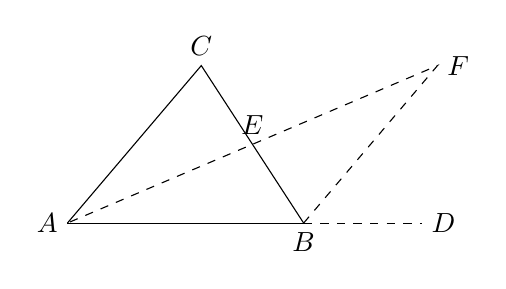
\begin{tikzpicture}[>=latex, scale=1]
\draw(0,0)node[left]{$A$}--(3,0)node[below]{$B$};
\draw[dashed](3,0)--(4.5,0)node[right]{$D$};
\draw(3,0)--(1.7,2)node[above]{$C$}--(0,0);
\draw[dashed](3,0)--(4.7,2)node[right]{$F$}--(0,0); 
\node at (2.35,1)[above]{$E$};
    \end{tikzpicture}
    \caption{}
    \end{minipage}
    \end{figure}

已知:$\triangle ABC$和外角
$\angle CBD$(图3.20)。

求证:$\angle CBD>\angle C$
或$\angle A$.

\begin{proof}
    假定$E$是$\overline{BC}$
中点,引$AE$并延长到$F$, 
使$\overline{EF}=\overline{AE}$, 作$\overline{BF}$.

在$\triangle ACE$和$\triangle FBE$中,

$\because\quad \overline{AE}=\overline{EF}$ (作图),

$\because\quad E$是$\overline{BC}$中点(假定),

$\therefore\quad \overline{CE}=\overline{EB}$(线段中点定义),

$\because\quad \angle CEA=\angle BEF$(对顶角相等),

$\therefore\quad \triangle ACE\cong \triangle FBE$ (SAS),

$\therefore\quad \angle EBF=\angle C$(全等三角形的对应角相等)。

由于$\angle CBD>\angle EBF$ (全量大于它的任何一部分)。

$\therefore\quad \angle CBD>\angle C$ (等量代换)。

同理可证 $\angle CBD> \angle A$.
\end{proof}

\begin{blk}{定理}
 在一个三角形中,如果两条边不等,那么它们所
对的角也不等,大边所对的角较大;反之,如果在一个三角
形中两个角不等,那么它们所对的边也不等。大角所对的边
较大。
\end{blk}

已知:$\triangle ABC$(图3.21)

\begin{figure}[htp]\centering
    \begin{minipage}[t]{0.48\textwidth}
    \centering
\begin{tikzpicture}[>=latex, scale=1.3]
\tkzDefPoint(0,0){A}
\tkzDefPoint(-50:2){C}
\tkzDefPoint(-120:2){D}
\tkzDefPoint(-120:3){B}
\tkzDefPoint(0,-1.5){O}
\tkzDrawPolygon(A,C,B)
\draw[dashed](D)--(C);
\tkzMarkAngles[mark=none, size=.3](C,D,A A,C,D)
\tkzLabelAngle[pos=.6](C,D,A){2}
\tkzLabelAngle[pos=.6](A,C,D){1}
\tkzAutoLabelPoints[center=O](A,C,B,D)       
    \end{tikzpicture}
    \caption{}
    \end{minipage}
    \begin{minipage}[t]{0.48\textwidth}
    \centering
    \begin{tikzpicture}[>=latex, scale=1.3]
\tkzDefPoint(0,0){A}
\tkzDefPoint(30:1.5){D}
\tkzDefPoint(-150:2){B}
\tkzDefPoint(-30:1.5){C}
\tkzDrawPolygon(A,C,B)
\draw[dashed](A)--(D)--(C);
\tkzMarkAngles[mark=none, size=.2](D,C,A A,D,C)
\tkzLabelAngle[pos=.4](A,D,C){2}
\tkzLabelAngle[pos=.4](D,C,A){1}
\tkzAutoLabelPoints[center=A](C,B,D)  
\node at (0,0)[above left]{$A$};
    \end{tikzpicture}
    \caption{}
    \end{minipage}
    \end{figure}

求证:
\begin{enumerate}
    \item $\overline{AB}>\overline{AC}\quad \Rightarrow\quad \angle C>\angle B$
    \item $\angle C>\angle B\quad \Rightarrow\quad \overline{AB}>\overline{AC}$
\end{enumerate}

\begin{proof}
    先证$\overline{AB}>\overline{AC}\quad\Rightarrow\quad \angle C>\angle B$.

在$AB$上截$\overline{AD}=\overline{AC}$,
则$\triangle ADC$为等腰三角形。

$\therefore\quad \angle 1=\angle 2$.

由于$\angle ACB>\angle 1$ (不等量基本性质6)

$\therefore\quad \angle ACB>\angle 2$(等量代换)。

但$\angle 2>\angle B$ (三角形的外角大于和它不相邻的任一内
角),

$\therefore\quad \angle ACB>\angle B$(不等量基本性质5)

即:$\angle C>\angle B$.

我们再证$\angle C>\angle B\quad \Rightarrow\quad \overline{AB}>\overline{AC}$

如果$\overline{AB}$不大于$\overline{AC}$, 那么$\overline{AB}=\overline{AC}$或$\overline{AB}<\overline{AC}$. 
若$\overline{AB}=\overline{AC}$, 则$\angle B=\angle C$, 若$\overline{AB}<\overline{AC}$,则$\angle C<\angle B$, 这两
种结果都和$\angle C>\angle B$矛盾。

$\therefore\quad \angle C>\angle B\quad \Rightarrow\quad \overline{AB}>\overline{AC}$
\end{proof}

\begin{blk}{定理}
    三角形任意两边之和大于第三边。
\end{blk}
 
已知:$\triangle ABC$(图3.23)。

求证:$\overline{AB}+\overline{AC}>\overline{BC}$.

\begin{proof}
    在$BA$的延长线上取一点$D$, 使$AD=AC$. 则
    $\triangle ACD$为等腰三角形。
  
    $\therefore\quad \angle 1=\angle 2$

    $\because\quad \angle BCD>\angle 1$(不等量
    基本性质6)

$\therefore\quad \angle BCD>\angle 2$(等量代
    换)。

    在$\triangle BCD$中,由前面的定理可知:
    $\overline{BD}>\overline{BC}$, 但$\overline{BD}=\overline{AB}+\overline{AD}=\overline{AB}+\overline{AC}$, 
 
   $\therefore\quad  \overline{AB}+\overline{AC}>\overline{BC}$
\end{proof}

\begin{blk}{推论}
三角形任一边大于其他两边之差。
\end{blk}

下面我们举例说明上述定理的一些应用。


\begin{example}
    已知:$\triangle ABC$中$\overline{AB}=\overline{AC}$, $D$点在$\overline{BC}$上,$E$点
在$\overline{BC}$的延长线上(图3.23)。

求证:$\overline{AD}<\overline{AB}<\overline{AE}$
\end{example}

\begin{figure}[htp]\centering
    \begin{minipage}[t]{0.48\textwidth}
    \centering
\begin{tikzpicture}[>=latex, scale=1]
    \tkzDefPoints{0/1.5/A, -1.5/-1/B, -.25/-1/D, 1.5/-1/C, 2.5/-1/E}
\tkzDrawPolygon(A,C,B)
    \draw(D)node[below]{$D$}--(A)node[above]{$A$}--(E)node[below]{$E$};
\draw[dashed](C)--(3.5,-1);
\node at (B)[below]{$B$};
\node at (C)[below]{$C$};
\tkzMarkAngles[mark=none, size=.3](D,B,A  A,D,B  A,C,B)
\tkzLabelAngle[pos=.5](D,B,A){1}
\tkzLabelAngle[pos=.5](A,D,B){3}
\tkzLabelAngle[pos=.5](A,C,B){2}
    \end{tikzpicture}
    \caption{}
    \end{minipage}
    \begin{minipage}[t]{0.48\textwidth}
    \centering
    \begin{tikzpicture}[>=latex, scale=1.2]
\tkzDefPoint(0,0){D}
\tkzDefPoint(-60:2){C}
\tkzDefPoint(180-60:1){A}
\tkzDefPoint(-140:1.2){E}
\tkzDefPoint(-140:2.8){B}
\tkzDrawPolygon(A,C,B)
\draw(B)--(E)--(C);
\draw[dashed](E)--(D);
\foreach \x in {A,D,C}
{
    \node at (\x) [right]{$\x$};
}
\foreach \x in {B,E}
{
    \node at (\x) [left]{$\x$};
}
\tkzMarkAngles[mark=none, size=.2](E,D,C)
\tkzLabelAngle[pos=.4](E,D,C){1}
    \end{tikzpicture}
    \caption{}
    \end{minipage}
    \end{figure}

\begin{proof}
$\because\quad \overline{AB}=\overline{AC}$

$\therefore\quad \angle 1=\angle 2$

又$\because\quad \angle 3>\angle 2$

$\therefore\quad \angle 3>\angle 1$

$\therefore\quad \overline{AB}>\overline{AD}$(在一个三角形中,大角对大边。)

又:$\because\quad \angle 2>\angle E$

$\therefore\quad \angle 1>\angle E$

$\therefore\quad \overline{AE}>\overline{AB}$(在一个三角形中,大角对大边。)

因此有:$\overline{AD}<\overline{AB}<\overline{AE}$
\end{proof}


\begin{example}
    已知:$E$点在$\triangle ABC$内(图3.24)。

求证: \begin{enumerate}
    \item $\angle BEC>\angle A$
    \item $\overline{BE}+\overline{EC}<\overline{AB}+\overline{AC}$
\end{enumerate} 
\end{example}

\begin{proof}
    延长$\overline{BE}$交$\overline{AC}$于$D$点,
则$\angle BEC>\angle 1$,$\angle BEC>\angle 1$

$\therefore\quad \angle BEC>\angle A$(不等量基
本性质5)。

又$\because\quad \overline{BE}+\overline{ED}<\overline{AD}+\overline{AB}$,$\overline{EC}<\overline{ED}+\overline{DC}$(三角形两边之和大于第三边)。

$\therefore\quad \overline{BE}+\overline{ED}+\overline{EC}<\overline{AD}+\overline{AB}+\overline{ED}+\overline{DC}$(不等量基本性质3)。

$\therefore\quad \overline{BE}+\overline{EC}<\overline{AB}+\overline{AC}$(不等量基本性质1)。
\end{proof}

\begin{example}
如图3.25所示,$A$、$B$是平面上直线$\ell$同侧的两点,
试在直线$\ell$上求一点$P$, 使$\overline{AP}+\overline{PB}$最短。

在没有作这题前,让我们想一想该怎样着手,我们要求
$\overline{AP}+\overline{PB}$最短,但怎样才能最短呢?

我们知道两点间的直线段最短,但是我们却要在$\ell$上求
一点,使$\overline{AP}+\overline{PB}$最短。如果$A,B$两点在$\ell$的两侧,那么问
题要简单得多(作$\overline{AB}$与$\ell$交于$P$, $P$点就是所求的点)。但
我们曾学过,如果两点是轴对称点,那么它们的对称轴就是
两点间线段的垂直平分线,并且对称轴上的点到两对称点的
距离相等。我们只要作出$A$点关于轴$\ell$的对称点$A'$, 我们求
$\overline{AP}+\overline{PB}$的最小值,就可转化为求$\overline{A'P}+\overline{PB}$的最小值了。
而$A'$、$B$两点在$\ell$的异侧,这是很容易的。

\begin{figure}[htp]
    \centering
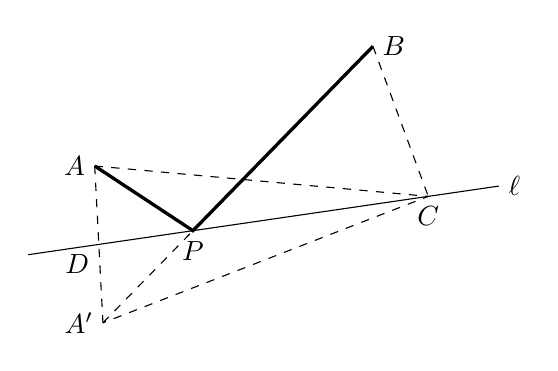
\begin{tikzpicture}[xscale=.6, rotate=5]
\draw (-2,0)--(8,0)node[right]{$\ell$};
\draw[dashed](-.5,1)node[left]{$A$}--(-.5,-1)node[left]{$A'$};
\draw[dashed](-.5,-1)--(5.5,2)node[right]{$B$};
\draw[very thick](-.5,1)--(1.5,0)node[below]{$P$}--(5.5,2);
\node at (-.5,0)[below left]{$D$};
\draw[dashed](-.5,1)  -- (6.5,0) node[below]{$C$}--(-.5,-1);
\draw[dashed](5.5,2)  -- (6.5,0);
\end{tikzpicture}
    \caption{}
\end{figure}
\end{example}


\begin{solution}
    作$A$点关于轴$\ell$的对称点$A'$, 作$\overline{A'B}$与$\ell$相交于$P$, 
    则$P$点使$\overline{AP}+\overline{PB}$最短。因为,如果在$\ell$上任找另外一点$C$, 
    在$\triangle A'BC$中,
    $\overline{A'B}<\overline{A'C}+\overline{CB}$(三角形两边之和大于第三边),
    但$\overline{A'B}=\overline{A'P}+\overline{PB}$

将    $\overline{A'P}=\overline{AP},\quad \overline{A'C}=\overline{AC}$ 代入上式,
    则得:$\overline{AP}+\overline{PB}<\overline{AC}+\overline{CB}$.

    这就证明了$P$点使$\overline{AP}+\overline{PB}$最短。
\end{solution}

\begin{rmk}
    如果$\ell$是镜子的话,那么从$A$点发出的光线,若反
射到$B$点,那么$\overline{AP}$、$\overline{PB}$就是光所走的路线。因为光线总是
走最近的路,在光学中就有:“入射角等于反射角”这条定
律。即$\angle APD=\angle BPC$. 在光学中由观测得到的结果和我
们用数学定理得出的结果一致。在自然界中我们有能力观测
到的结论是有限的,如何由这些有限的可观测的结论,得到
更进一步的结论,甚至有些是观测不到的结论,我们需要数
学这样有力的工具。
\end{rmk}
    
\begin{ex}
\begin{enumerate}
    \item 已知:如图,$\triangle ABC$内有一点$P$, 
    求证:$\angle BPC>\angle BAC$.
    \item 已知:如图,$\triangle ABC$内有一点P,
    求证:$\overline{AB}+\overline{AC}>\overline{PB}+\overline{PC}$.
    \item 将金属丝弯成三角形,如果要求一边长是25cm, 那么
    金属丝至少大于多少cm才能作成三角形?
    \item 证明四边形两条对角线之和小于周长而大于半周长。
 \item 证明三角形的一边小于它的周长的一半。
 \item  用整数表示三角形的各边,一边是3米,另一边是2米,第
    三边可以是多少米?
\item  在平面上$\overline{AB}$
    的垂直平分线的$A$点的一侧取一点$P$, 那
    么$\overline{PA}$和$\overline{PB}$哪一条线段长?
\item 已知:如图,$\triangle ABC$中,
$\angle A>\angle C$, $D$、$E$分别在$\overline{AB}$、
    $\overline{AC}$上并且$\overline{AD}>\overline{AE}$.
    求证:
    \begin{enumerate}
        \item $\angle BDE> \angle CED$
        \item $\overline{BC}>\overline{BE}$
    \end{enumerate}
\end{enumerate}
\end{ex}
    
\begin{figure}[htp]\centering
    \begin{minipage}[t]{0.48\textwidth}
    \centering
\begin{tikzpicture}[>=latex, scale=1]
    \tkzDefPoint(-60:2){C}
    \tkzDefPoint(180-60:1){A}
    \tkzDefPoint(-140:2.8){B}
    \tkzDefPoint(-.25,-.5){P}
    \tkzDrawPolygon(A,C,B)
    \draw(B)--(P)--(C);
\tkzAutoLabelPoints[center=P](A,B,C)
\node at (P)[above]{$P$};
    \end{tikzpicture}
    \caption*{第1--2题}
    \end{minipage}
    \begin{minipage}[t]{0.48\textwidth}
    \centering
    \begin{tikzpicture}[>=latex, scale=1.3]
        \tkzDefPoint(0,0){A}
        \tkzDefPoint(-45:2){C}
        \tkzDefPoint(-45:1){E}
        \tkzDefPoint(-140:2.8){B}
        \tkzDefPoint(-140:2){D}
        \tkzDrawPolygon(A,C,B)
        \tkzDrawPolygon(D,B,E)
        \tkzDefPoint(.1,-1){O}
        \tkzAutoLabelPoints[center=O](A,B,C,D,E)

    \end{tikzpicture}
    \caption*{第8题}
    \end{minipage}
    \end{figure}


\begin{example}
    
\end{example}

\begin{solution}
    
\end{solution}
\begin{example}
    
\end{example}

\begin{example}
    
\end{example}

\begin{solution}
    
\end{solution}
